\documentclass[border=4pt]{standalone}
\usepackage[T1]{fontenc}
\usepackage{helvet}
\renewcommand{\familydefault}{\sfdefault}
\usepackage{graphicx}
\usepackage{caption}
\usepackage{amsmath}
\captionsetup{font={sf,footnotesize},labelfont={sf,bf,footnotesize},justification=justified,singlelinecheck=false}
\begin{document}
\setcounter{figure}{3}
\begin{minipage}{7.20in}
\centering
\begin{figure}[htbp]
    \centering
    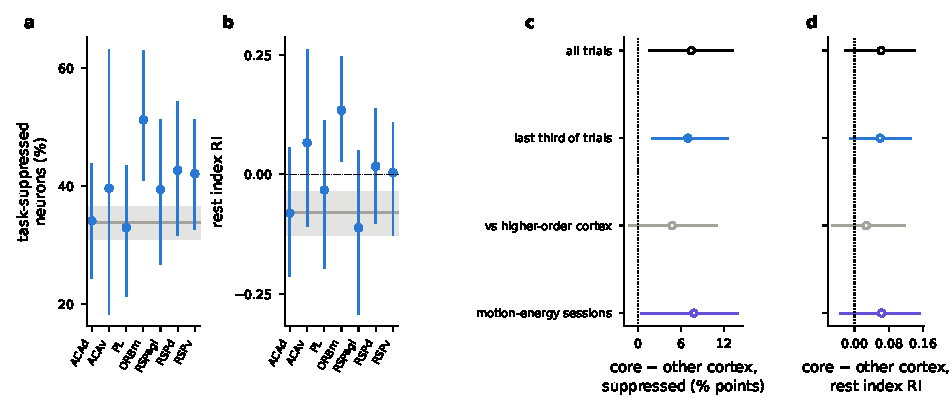
\includegraphics[width=\linewidth]{fig4_restpref_panels.pdf}
    \caption{\textbf{a} Percentage of neurons per cortical region (Beryl) significantly suppressed during the task (movement onset, movement and feedback windows) relative to still 0.3 s chunks of the grey-screen period (Welch test with one chunk per 3 s, p $<$ 0.01; 53,213 neurons, 395 sessions, 130 mice). Colour: the conservative DMN core (ACA, RSP, PL, ORBm; Fig. 1), regions assigned to the DMN by at least one of the four papers but not in the core, and regions in none. \textbf{b} Per region, the same measure referenced to task ITIs (earlier report) against the grey-screen reference; Spearman $\rho$ = 0.44 over 43 regions. \textbf{c} Difference between the conservative core (and, for comparison, the full Whitesell et al. and Lu et al. sets) and all other cortex in the suppressed fraction (left) and in the continuous rest index RI = (rest $-$ task)/(rest + task) (right), against all trials (black) or only the last third of trials, closest in time to the grey screen (blue): 95\% mouse-bootstrap CI; filled markers, region-permutation p $<$ 0.05. Note that 81\% of neurons differ significantly between grey screen and task, so the suppressed fraction is close to the sign of RI.}
    \label{fig:grey_restpref}
\end{figure}
\end{minipage}
\end{document}
